\section{IMU测量模型}
\subsection{加速度计测量原理}
\subsection{陀螺仪的测量原理}

%%%%%%%%%%%%%%%%%%%%%%%%%%%%

\begin{frame}
  \frametitle{加速度计测量原理 \hfill 
\includegraphics[height=0.5cm]{00_logo.png}}
  \begin{columns}
    \column{0.1\textwidth}
    
    \column{0.5\textwidth}
    \begin{itemize}
      \item 其测量原理可以用一个质量块+弹簧+指示计来表示.
      \item 加速度计测量值$a_m$为弹簧拉力对应的加速度,
        \begin{equation}
          a_m = \frac{f}{m} = a - g
        \end{equation}
      
      其中,f为弹簧拉力, a为物体在惯性系下的加速度,g为重力加速度.
      
      \item 通过受力影响位移,位移影响电容大小,通过测量电流的方式获得$a_m$

    \end{itemize}

    \column{0.3\textwidth}
    \begin{figure}[h]
      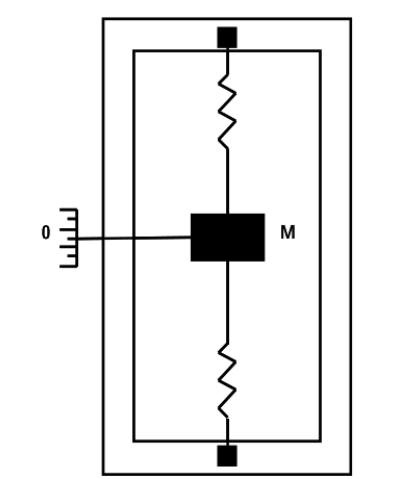
\includegraphics[trim=1.5 0 0 0, height=3.5cm,clip]{12_0.png}
      % \caption{四个区域搜索空间}
    \end{figure}

    \column{0.1\textwidth}
  
  \end{columns}
  \end{frame}    


%%%%%%%%%%%%%%%%%%%%%%%%%%%%

\begin{frame}
  \frametitle{陀螺仪测量原理 \hfill 
\includegraphics[height=0.5cm]{00_logo.png}}
  \begin{columns}
    \column{0.1\textwidth}
    
    \column{0.5\textwidth}
    \begin{itemize}
      \item 陀螺仪主要用来测量物体的旋转角速度,按测量原理分有震动陀螺/光纤陀螺等.

      \item 一般采用震动陀螺原理,通过测量Coriolis force 来间接得到角速度.
      
      \item 一个主动运动轴 + 一个敏感轴

    \end{itemize}
    
    \column{0.3\textwidth}
    \begin{figure}[h]
      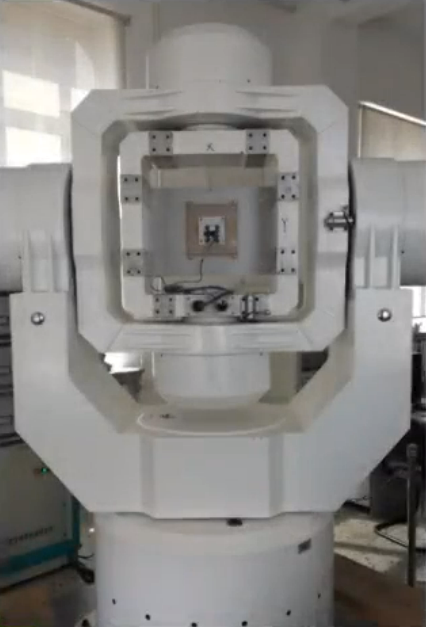
\includegraphics[trim=1.5 0 0 0, height=3.5cm,clip]{12_1.png}
      % \caption{四个区域搜索空间}
    \end{figure}

    \column{0.1\textwidth}
  
  \end{columns}
  \end{frame}    

%%%%%%%%%%%%%%%%%%%%%%%%%%%%

\begin{frame}
  \frametitle{音叉振动陀螺原理 \hfill 
\includegraphics[height=0.5cm]{00_logo.png}}
  \begin{columns}
    \column{0.1\textwidth}
    
    \column{0.8\textwidth}
    \begin{itemize}
      \item 音叉中间为旋转轴,音叉左右两个质量块,做方向相反的正弦运动,质量块受到的科氏力方向相反.
      \item 为什么要这么做?一个质量块行不行?

    \end{itemize}
    
    % \column{0.4\textwidth}
    \begin{figure}[h]
      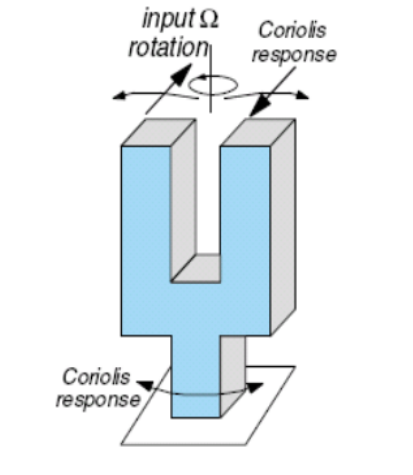
\includegraphics[trim=1.5 0 0 0, height=3.5cm,clip]{12_2.png}
      \qquad
      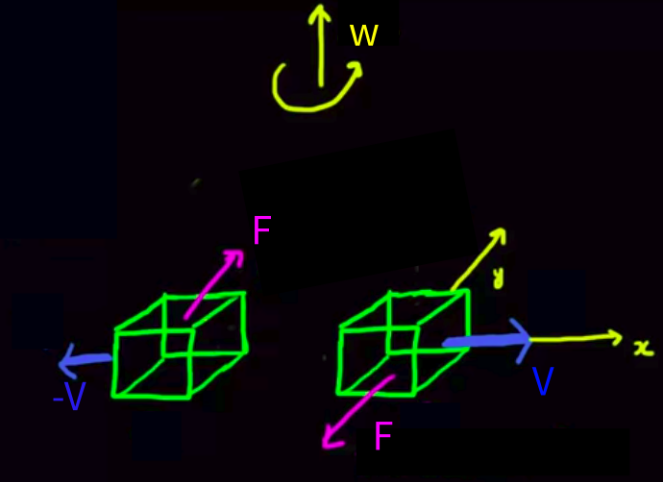
\includegraphics[trim=1.5 0 0 0, height=3.5cm,clip]{12_3.png}
      % \caption{四个区域搜索空间}
    \end{figure}

    \column{0.1\textwidth}
  
  \end{columns}
  \end{frame}    

%%%%%%%%%%%%%%%%%%%%%%%%%%%%

\begin{frame}
  \frametitle{思考 \hfill 
\includegraphics[height=0.5cm]{00_logo.png}}
  \begin{columns}
    \column{0.1\textwidth}
    
    \column{0.8\textwidth}
    \begin{itemize}
      \item 实际上,两个质量块不可能完全一致,也就是说陀螺仪的测量会受到外部加速度的影响,即常称的G-sensitivity.
      
      \item 加速度计不需要考虑科氏力的影响吗?

    \end{itemize}
    

    \column{0.1\textwidth}
  
  \end{columns}
  \end{frame}    